\par
Biblioteka Qt, rozwijana przez organizacje Qt Project, jest zbiorem bibliotek i narzędzi programistycznych dedykowanych dla języków C++, QML i Java.
\par
Qt jest głownie znane jako biblioteka do tworzenia interfejsu graficznego, jednakże posiada ona wiele innych rozwiązań ułatwiających programowanie obiektowe i zdarzeniowe.
\par
Wybrałem Qt z uwagi na to, że posiada interfejs w C++.
Oraz kompilacja oprogramowania używającego Qt może odbywać się za pomocą dwóch narzędzi: CMake oraz dedykowanego narzędzia qmake, zrobionego specjalnie na potrzeby biblioteki Qt.
Dzięki czemu cały projekt przeglądarki używa tego samego języka oraz tego samego narzędzia zarządzania kompilacją.

\subsection{Wymowa}

\par
Według autorów, Qt powinno się czytać jak angielskie słowo \enquote{cute}, po polsku \enquote{kiut}.
Jednakże społeczność programistów nie jest co do tego zgodna.
Ankiety zrobione na dwóch popularnych serwisach internetowych o tematyce programistycznej, pokazują, że najbardziej popularną wymową jest \enquote{Q.T.}, po polsku \enquote{ku te}.
\par
Odnośniki do przytoczonych ankiet:
\begin{itemize}
    \item \url{https://ubuntuforums.org/showthread.php?t=1605716}
    \item \url{https://www.qtcentre.org/threads/11347-How-do-you-pronounce-Qt}
\end{itemize}

\subsection{Licencja}

\par
Biblioteka Qt jest dystrybuowana w dwóch wersjach: komercyjnej i otwarto źródłowej.
Wersja otwarto źródłowa nie posiada wielu modułów, ale jest dystrybuowana na licencji \href{https://www.gnu.org/licenses/gpl.html}{GNU General Public License w wersji 3}.
Co sprawia, że bibliotekę można użyć w mojej pracy.

\subsection{Normy i certyfikaty}

\par
The Qt Company posiada szereg certyfikatów od FDA i UE, ułatwiające wprowadzenie produktów używających bibliotek Qt na rynek Europejski jak i Amerykański.
\par
Lista posiadanych norm:
\begin{itemize}
    \item IEC 62304:2015 (2006 + A1)
    \item IEC 61508:2010-3 7.4.4 (SIL 3)
    \item ISO 9001:2015 
\end{itemize}
Więcej informacji na temat certyfikatów można przeczytać na oficjalnej stronie Qt pod adresem \url{https://www.qt.io/qt-in-medical/}.

\subsection{Globalne typy struktur}
\label{sec:qt-typedefs}
\par
W różnych systemach operacyjnych są różne kompilatory i w śród tej różnorodności pojawia się problem dotyczący zmiennych fundamentalnych.
Na przykład: Ile bitów ma zmienna \cppcode{int}?
Udając się do oficjalnej dokumentacji C++, dostępnej pod adresem \url{https://pl.cppreference.com/w/cpp/language/types}, możemy dowiedzieć się, że \cppcode{int} ma minimum 16 bitów.
Natomiast w dokumentacji MSVC, kompilatora firmy Microsoft, znajdującej się pod adresem \url{https://docs.microsoft.com/pl-pl/cpp/cpp/int8-int16-int32-int64?view=vs-2019}, widnieje informacja z której wynika, żeby mieć pewność o długości liczby całkowitej należy użyć takich typów: \cppcode{\_\_int8}, \cppcode{\_\_int16}, \cppcode{\_\_int32}, \cppcode{\_\_int64}.
\par
Jest to problem, który biblioteka Qt rozwiązała.
Wprowadziła dodatkowe typy literałów, które dostosowują się do systemu i kompilatora i zapewniają pewność podczas deklaracji, że dana zmienna będzie zakładanej długości.
Dodatkowe typy literałów są dostępne w nagłówku \cppcode{<QtGlobal>}, dokumentacja dostępna pod adresem \url{https://doc.qt.io/qt-5/qtglobal.html}.

\par
Dlatego w pracy zostały użyte typu fundamentalne dostarczane przez bibliotekę Qt.
Kilka przykładów:
\begin{itemize}
    \item \cppcode{qint8} --- liczba całkowita, 8 bitowa, ze znakiem
    \item \cppcode{qint16} --- liczba całkowita, 16 bitowa, ze znakiem
    \item \cppcode{qint32} --- liczba całkowita, 32 bitowa, ze znakiem
    \item \cppcode{qint64} --- liczba całkowita, 64 bitowa, ze znakiem
    \item \cppcode{quint8} --- liczba całkowita, 8 bitowa, beq znaku
    \item \cppcode{quint16} --- liczba całkowita, 16 bitowa, beq znaku
    \item \cppcode{quint32} --- liczba całkowita, 32 bitowa, beq znaku
    \item \cppcode{quint64} --- liczba całkowita, 64 bitowa, beq znaku
    \item \cppcode{qreal} --- największa dostępna liczba zmiennoprzecinkowa
\end{itemize}

\subsection{Klasa QObject}

\qtclassExplanations

\par
Biblioteka Qt implementuje klasę \qtclass{QObect}, która jest bazą dla wszystkich obiektów Qt i wszystkie klasy współpracujące z biblioteką Qt powinny po niej dziedziczyć.
\qtclass{QObject} implementuje 2 podstawowe rzeczy: system drzewa obiektów (opisany w sekcji \ref{sec:qt-pareting}), system sygnałów (opisany w sekcji \ref{sec:qt-signals}).

\subsubsection{Drzewa obiektów}
\label{sec:qt-pareting}

\par
W C++ jednym z największych problemów jest wyciek pamięci, pojawia się wtedy gdy zaalokujemy na stercie ony obiekt za pomocą operatora \cppcode{new} i nie go usunąć gdy ten będzie potrzebny.
\par
\qtclass{QObject} zakłada, że obiekty mogą mięć jednego rodzica, a rodzic może mieć wiele dzieci.
Rodzica można przypisać podczas tworzenia obiektu oraz zmieniać go dowolnie w trackie działania programu.
Przypisanie rodzica dziecku oznacza to, że gdy wywołamy destruktor rodzica, ten wywoła destruktory dzieci i w ten sposób całe drzewo obiektów zostanie zniszczone.
\par
Mechanizm ten pozwala nam tworzyć nowe obiekty na stercie i nie martwić się o ich poźniejsze sprzątnięcie.
Jest to o tyle efektywne, że nie trzeba dla każdego obiektu tworzyć odrębnego wskaźnika lub wektora wskaźników w deklaracji klasy, a dzięki temu można mieć czystszy i czytelniejszy kod źródłowy.
Przykładowe użycie:
\par
\begin{lstlisting}[language=C++]
int main() {

    // Tworzymy obiekt przycisku
    auto *quit = new QPushButton("Quit");
    // Tworzymy obiekt okna
    auto *window = new QWidget();

    // Przypisujemy rodzica przyciskowi
    quit->setParent(window);
    
    ...

    // W tym momencie przycisk wraz z oknem zostaja usuniete
    delete window;
}
\end{lstlisting}

\subsubsection{Sygnały i sloty}
\label{sec:qt-signals}

\par
System sygnałów i slotów jest implementacją programowania zdarzeniowego.
Sygnał jest źródłem zdarzenia, a slot jest odbiornikiem zdarzenia.
Sygnał obiektu jest łączony do slotu obiektu dynamicznie w czasie działania programu.
Do jednego sygnału można podłączyć wiele slotów, jak i do jednego slotu można wprowadzić wiele sygnałów.
Gdy zdarzenie zostanie wyemitowane, to wszystkie sloty podłączone do sygnału zostaną powiadomione.
Sygnały i sloty są implementowane przez funkcje definiowane w deklaracji klasy.
System sygnałów Qt nie ma nic wspólnego w sygnałach pojawiających się w C, takich jak \enquote{SIGTERM}.
Dodatkowo sygnały w Qt są wstanie przenosić argumenty definiowane przez programistę.
Taka implementacja umożliwia programowanie zdarzeniowe.

\par
Przykład użycia sygnałów do propagacji zdarzenia.

\begin{lstlisting}
/* Tworzymy dwa obiekty klasy Counter (definicja w następnej sekcji) */
Counter a, b;

/* Łączymy sygnał Counter::valueChanged obiektu "a",
   do slotu Counter::setValue obiektu "b" */
QObject::connect(&a, &Counter::valueChanged,
                 &b, &Counter::setValue);

/* Ustawiamy wartość licznika obiektu "a" na 12 */
a.setValue(12);

/* W czasie ustawiania został wysłany sygnał z "a" do "b", więc:
   a.value() == 12    b.value() == 12 */

/* Ustawiamy wartość licznika obiektu "b" na 48 */
b.setValue(48);

/* Sygnał Counter::valueChanged obiektu "b" nie jest podłączony do
   żadnego slotu, więc:
   a.value() == 12     b.value() == 48 */

\end{lstlisting}

\par
Pełna dokumentacja na temat sygnałów i slotów znajduje się na oficjalne stronie Qt pod adresem \url{https://doc.qt.io/qt-5/signalsandslots.html}

\subsubsection{Przykładowa klasa dziedzicząca po QObject}
\begin{lstlisting}[language=C++]
#include <QObject>

class Counter : public QObject {
    /* Każdy klasa dziedzicząca po QObject musi na samym
        początku swojej definicji mieć makro "Q_OBJECT". */
    Q_OBJECT

public:
    Counter() { m_value = 0; }

    int value() const { return m_value; }

    /* Sloty powinny być poprzedzone makrem "slots".
        Widoczność slotów można zmieniać. */
public slots:
    void setValue(int value){
        if (value != m_value) {
            m_value = value;

            /* Podczas wywoływania sygnału należy
                poprzedzić to makrem "emit". */
            emit valueChanged(value);
        }
    }

    /* Sygnały powinny być poprzedzone makrem "signals".
        Wszystkie sygnały są publiczne. */
signals:
    void valueChanged(int newValue);

private:
    int m_value;
};

\end{lstlisting}

\subsection{Graficzny interfejs użytkownika}
\label{sec:qt-gui}
\par
Graficzny interfejs użytkownika został zaimplementowany za pomocą klasy \qtclass{QWidget}.
Klasa ta dziedziczy po \qtclass{QObject} i po \qtclass{QPaintDevice}, obiekcie służącym do rysowania.
\qtclass{QWidget} reprezentuje element graficzny interfejsu użytkownika, ma zaimplementowany mechanizm renderowania, wyświetlania na ekranie użytkownika, obsługi myszki klawiatury, przeciągnięcia i upuszczenia \fromEng{drag and drop}, itp.
Wszystkie elementy takie jak przyciski i pola tekstowe muszą dziedziczyć po niej.
\par
Interfejs klasy jest niezależny od platformy na, której się znajduje.
Nawet tworzenie własnej, niestandardowej kontrolki nie wymaga uwzględniania systemu operacyjnego, a przynajmniej w kwestii użytkowej.

\begin{figure}[!htbp]
    \centering
    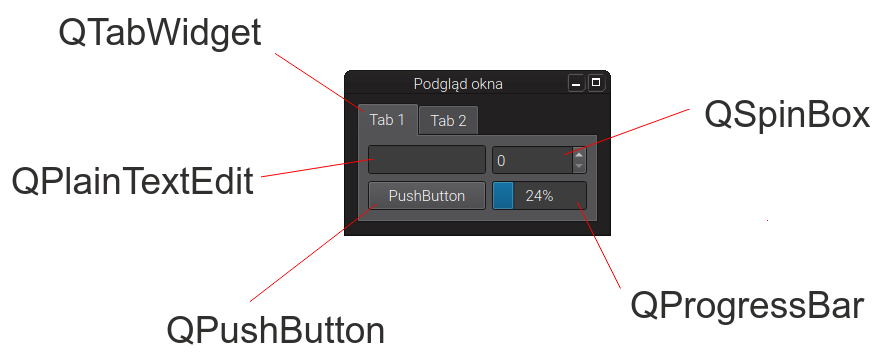
\includegraphics[width=\textwidth]{img/qt-gui-001.png}
    \caption{Przykładowe okienko programu w Qt. Zdjęcie własne.}
    \label{fig:qtgui1}
\end{figure}

\par
Kilka przykładowych klas obiektów graficznych i ich cechy
\begin{itemize}
    \item \qtclass{QLabel} --- klasa służąca do wyświetlania tekstu bez możliwości interakcji z nim.
          Dziedziczy po klasie \qtclass{QFrame}, która dziedziczy po \qtclass{QWidget}.

    \item \qtclass{QPushButton} --- klasa do tworzenia zwykłego przycisku.
          Dziedziczy po klasie \qtclass{QAbstractButton}, która dziedziczy po \qtclass{QWidget}.
          Obsługa zdarzenia wciśnięcia przycisku jest przez obsługę sygnału \qtfunction{QAbstractButton}{clicked}.
          Przykład można zobaczyć na przykładowym rysunku \ref{fig:qtgui1}.

    \item \qtclass{QTabWidget} --- implementuje zakładki, takie jak w przeglądarce internetowej.
          Dziedziczy bezpośrednio po klasie \qtclass{QWidget}.
          Zawartości zakładek mogą być zwykłymi obketami dziedziczącymi po \qtclass{QWidget}.
          Przykład można zobaczyć na przykładowym rysunku \ref{fig:qtgui1}.

    \item \qtclass{QPlainTextEdit} --- implementuje pole umożliwiające wprowadzanie teksu rzez użytkownika.
          Dziedziczy po klasie \qtclass{QAbstractScrollArea}, które dziedziczy po  \qtclass{QFrame}, z kolei ta po \qtclass{QWidget}.
          Przykład można zobaczyć na przykładowym rysunku \ref{fig:qtgui1}.

    \item \qtclass{QProgressBar} --- implementuje pasek postępu w dwóch wersjach poziomej i pionowej.
          Dziedziczy bezpośrednio po klasie \qtclass{QWidget}.
          Przykład poziomego paska można zobaczyć na przykładowym rysunku \ref{fig:qtgui1}.

    \item \qtclass{QSpinBox} --- implementuje prządkę, czyli kontrolkę przystosowaną do wprowadzania liczb przez użytkownika.
          Posiada dwa dodatkowe przyciski pozwalające w łatwy sposób zwiększyć lub zmniejszyć zawartość.
          Przykład można zobaczyć na przykładowym rysunku \ref{fig:qtgui1}.

\end{itemize}

\subsection{Oddzielenie od platformy}

Biblioteka standardowa

Własne wektroy

Własne wątki
